\SetKwProg{Proc}{procedure}{}{}
\SetKwFunction{Search}{SEARCH}
\SetKwFunction{SampleParticle}{SAMPLE-PARTICLE}
\SetKwFunction{Simulate}{SIMULATE}
\SetKwFunction{Timeout}{TIMEOUT}
\SetKwFunction{Maxstep}{MAX-STEP}
\SetKwFunction{SearchBest}{SEARCH-BEST}
\SetKwFunction{UCB}{UCB}
\SetKwFunction{Rollout}{ROLLOUT}

\SetKwFunction{BeliefUpdate}{UPDATE}
\SetKwFunction{ComputeConfidence}{CONF}
\SetKwFunction{SelectBestHypothesis}{SELECT-HYPO}
\SetKwFunction{QueryFM}{QUERY-FM}
\SetKwFunction{FilterBelief}{FILTER}
\SetKwFunction{Planning}{PLANNING}



\section{System Architecture and Methods}~\label{method:system_architecture}
In this section, we present an overview of the system architecture and the data flows between modules. Then we give a detailed explanation of their functionalities and applications.

\begin{figure*}[t!]
\captionsetup{skip=0pt}
    \centering
    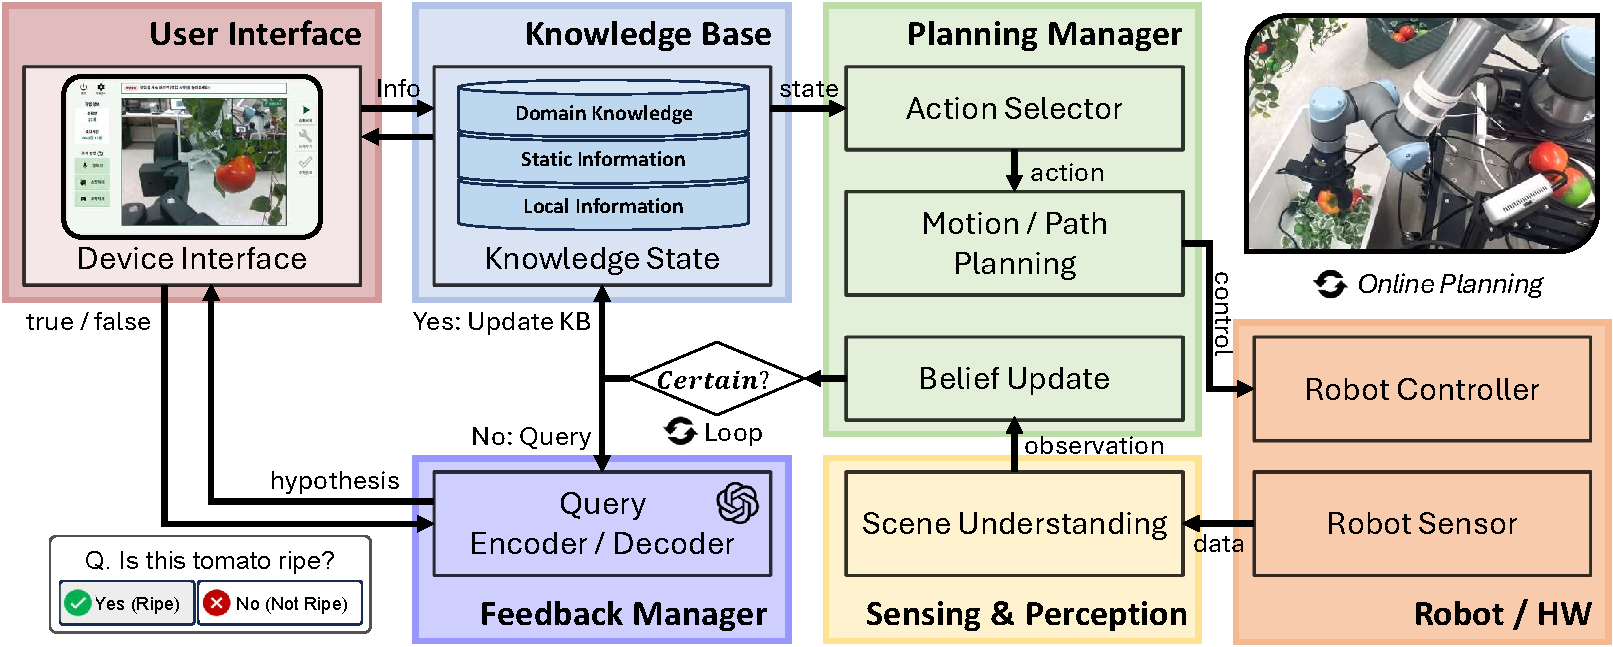
\includegraphics[width=0.95\linewidth]{figures/intro_and_method/fig_dataflow.pdf}
    \caption{System architecture and data flow of the proposed framework. The system consists of the \textit{Knowledge Base} (KB), \textit{Planning Manager} (PM), \textit{Sensing and Perception} module (SP), \textit{Feedback Manager} (FM), and \textit{User Interface} (UI). The PM performs online planning based on the current knowledge state stored in the KB and updates the belief using observations from SP. The system evaluates the confidence of the updated belief. If the confidence exceeds a threshold, the most probable hypothesis is committed to the KB. Otherwise, the FM generates a query and requests corrective feedback from the user through the UI. The feedback is then used to refine the belief and continue planning.}
    \label{fig:data_flow}
    % \vspace{-10pt}
\end{figure*} 


\subsection{Overview}~\label{method:overview}
Fig.~\ref{fig:data_flow} illustrates the brief system architecture and the data flow between the main modules. We integrate the \textit{Knowledge Base} (KB), the \textit{Planning Manager} (PM), the \textit{Sensing and Perception} module (SP), the \textit{Feedback Manager} (FM), and the \textit{User Interface} (UI). The KB maintains symbolic descriptions and facts used for planning, SP generates sensory information from robot sensors, PM generates and executes plans, FM coordinates corrective feedback, and UI bridges the system and the user. 

The KB stores essential information required for the robot to perform tasks and explicitly represents the current state of the system. All modules share information and interact with each other through the KB. The KB is composed of three types of information: domain knowledge, static information, and local information. Domain knowledge refers to prior knowledge in a specific domain. It includes descriptions of robot skills, domain-specific rules, and general explanations of the environment. Static information is used during planning and execution but remains unchanged throughout task execution. Unlike domain knowledge, static information is encoded in a structured form and includes information such as robot parameters and local maps. In contrast, local information is used during planning and execution but cannot be known in advance. It is obtained through observations from the SP module and stored in the KB in the form of facts. 


The PM is responsible for online action selection and execution under partial observability. The POMCP-based planner within the PM module selects the best action from the current belief and triggers the SP module to acquire additional observations. For instance, if the robot is positioned in front of a tomato stem, it naturally executes a \texttt{detect} action to infer the locations and ripeness states of tomatoes. To quantify uncertainty, the PM approximates the belief in the form of particle and computes the entropy over the resulting belief distribution. If such uncertainty is detected, the PM queries the FM to obtain additional information that can resolve the ambiguity of the observation. Upon receiving a response from the FM, the PM updates the belief accordingly and promotes the most probable belief state to a certain state in the knowledge base.


The SP module provides the current visual sensing information to the UI in real time. In addition, it updates the KB with observations triggered by the PM. In this process, the SP module makes use of data from various sensors, such as cameras, LiDAR, and tactile sensors, to extract information used for task execution, including object locations, states, and properties. For example, from RGBD images, the SP module infers visual attributes such as the position, ripeness, and state of a tomato, while tactile sensors are used to perceive contact-based properties such as object stiffness or softness. The high-level perceptual information extracted by the SP module is stored in the KB in the form of symbolic facts.

% FM modules
The FM module converts symbolic hypotheses from the PM into user-facing questions using a predefined predicate-to-template mapping. For example, a hypothesis such as $\texttt{ripe}(\text{tomato}_1)$ is mapped to a question such as ``Is tomato 1 ripe?''. Along with the query, the UI highlights the referenced object with a bounding box. The FM then maps the response from the user to a boolean value, which is used by the PM to filter the belief.

Finally, the UI displays the current visual sensing information and the system state, and allows the user to provide direct feedback or make selections. The user interacts with the FM module through the UI to monitor and supervise task execution.




% \newpage
\subsubsection{Knowledge Base}~\label{method:KB}
The KB maintains a structured representation of the environment, including objects, properties, task-relevant relations, numeric quantities, and their associated confidence values. Formally, we define $\mathcal{KB} = \mathcal{I}^{D} \sqcup \mathcal{I}^{S} \sqcup \mathcal{I}^{L}$,\footnote{The notation $\sqcup$ denotes a disjoint union, indicating that $\mathcal{I}^{D}$, $\mathcal{I}^{S}$, and $\mathcal{I}^{L}$ form a partition of $\mathcal{KB}$.} where $\mathcal{I}^{D}$, $\mathcal{I}^{S}$, and $\mathcal{I}^{L}$ denote the domain, static, and local information sets, respectively, as described in Sec.~\ref{method:overview}.

For $\mathcal{I}^{S}$ and $\mathcal{I}^{L}$, each information set contains both symbolic facts and numeric fluents. A symbolic fact is defined as $f = \text{pred}(\mathbf{x})$, where $\text{pred}(\cdot)$ denotes a predicate symbol and $\mathbf{x}$ denotes its arguments. A numeric fluent is defined as $\nu = \langle g(\mathbf{x}), v \rangle$, where $g(\mathbf{x})$ denotes a numeric function over objects and $v \in \mathbb{R}$ denotes its value. For example, symbolic facts can represent object categories and relations, such as $\texttt{tomato}(\text{tomato}_1)$ and $\texttt{loc}(\text{stem}_1)$, while numeric fluents can represent measurable quantities, such as $\texttt{pose\_x}(\text{tomato}_1)=0.12$ or $\texttt{distance}(\text{robot}, \text{stem}_1)=2.5\ (m)$.


Specifically, the set $\mathcal{I}^{S}$ contains information that remains invariant throughout planning. By definition, for all $a \in \mathcal{A}$, $\mathrm{Effect}(a) \cap \mathcal{I}^{S} = \emptyset$, where $\mathrm{Effect}(a)=\mathrm{add}(a) \cup \mathrm{del}(a)$ denotes symbolic effects and can be extended to include numeric updates. These elements capture structural properties of the environment that are not altered by any action. For example, predicates such as $\texttt{tomato}(\text{tomato}_1)$ and $\texttt{loc}(\text{stem}_1)$, as well as fixed numeric quantities like $\texttt{loc\_x}(\text{stem}_1)=1.2$, remain unchanged regardless of the executed actions.


In contrast, $\mathcal{I}^{L}$ denotes local information obtained through the SP module and is not known a priori. This includes perceptual predicates, such as object existence or category estimates, as well as numeric fluents estimated from sensor data. For example, predicates such as $\texttt{ripe}(\text{tomato}_1)$ or $\texttt{detected}(\text{tomato}_2)$ may be inferred from observations, and numeric values such as $\texttt{distance}(\text{robot}, \text{stem}_1)=2.3$ or $\texttt{pose\_x}(\text{tomato}_1)=-0.5$ are updated as new sensor measurements become available.


\subsubsection{Planning Manager}~\label{method:PM}
The PM performs decision making based on the current belief state while continuously updating the knowledge base during execution, as illustrated in Fig.~\ref{fig:pm}. Uncertainty is quantified using the entropy of the belief distribution. If the uncertainty exceeds a threshold, the planner requests additional verification from the FM. Otherwise, it commits the most probable hypothesis to the knowledge base and proceeds with action execution. In the following, we describe the belief approximation, the uncertainty estimation, the POMCP based search, and the overall planning procedure.


\begin{figure}[t]
\captionsetup{skip=0pt}
\centering

\includegraphics[width=0.98\linewidth]{figures/intro_and_method/fig_overview.pdf}
\caption{Planning Manager workflow. The PM maintains a belief over symbolic possible worlds, updates it using observations, and evaluates belief uncertainty. If uncertainty exceeds a threshold, the PM requests verification through the FM. Otherwise, it commits the most probable hypothesis to the KB and continues planning and execution.}
\label{fig:pm}
\end{figure}


% A history is a sequence of actions and observations
\paragraph{Belief representation}~\label{method:belief_rep}
In partially observable environments, the true state cannot be directly observed, and thus the PM maintains a belief, which is a probability distribution over states. The belief at time $t$ is defined as $b_t(s) = P(s_t = s \mid h_t)$, where $h_t = \{a_1, o_1, \dots, a_t, o_t \}$ denotes the history of actions and observations. However, in symbolic domains, the state space is large and subject to structural constraints, making exact belief tracking computationally intractable. Thus, we approximate the belief using a set of particles.

Formally, at time step $t$, the belief is represented as a finite set of particles and their associated weights:
\[
\mathcal{B}_t = \{ (s_i, w_i) \}_{i=1}^{N}, \quad \sum_{i=1}^{N} w_i = 1,
\]
where each $s_i$ denotes a possible world composed of a finite set of facts. The approximated belief distribution is then
\[
b_t(s) \approx \sum_{i=1}^{N} w_i \, \delta(s_i = s).
\]


In the symbolic domain, actions exhibit partially predictable effects due to their interpretable structure. For example, $\texttt{pick}(\text{tomato}_1)$ may result in grasp failure or selecting a different tomato while leaving the robot location unchanged. Based on this observation, we define a finite set of distinct reachable successor states, referred to as the \textit{frontier}. For each $s$ and $a$, the frontier is defined as
\[
Frontier(s,a) = \{ s_1^{\star}, s_2^{\star}, \dots, s_j^{\star} \},
\]

where each $s_k^{\star}$ denotes a reachable successor state and $s_k^\star \neq s_\ell^\star$ for $k \neq \ell$.


The frontier is generated from the symbolic transition model $T(s^\prime \mid s,a)$ by applying action $a$ to the current state. We use the STRIPS-style action representation introduced in Sec.~\ref{preliminaries:STRIPS}, and action selection is restricted to actions applicable in the sampled symbolic state. Deterministic effects are applied directly. For uncertain perceptual or execution effects, the action model enumerates the possible symbolic successors with nonzero transition probability. Thus, the frontier is the finite support of $T(\cdot \mid s,a)$ under the symbolic transition model, and the prior frontier weight is given by $w_k = T(s_k^\star \mid s,a)$. For example, an applicable $\texttt{pick}(\text{tomato}_1)$ action may produce a success successor with probability $0.8$, in which the symbolic effect of picking is added to the state, and a failure successor with probability $0.2$, in which the robot remains in a hand-empty state. These successors become elements of $Frontier(s,a)$ with prior weights $0.8$ and $0.2$, respectively. 

In contrast to standard particle filtering, we assume a \textit{knowledge} state $s^{K}$ that represents the set of certain facts. Given $a$ and $s^{K}$, we construct the belief by considering only the reachable states induced by $s^{K}$. That is, particles are defined exclusively over the frontier $Frontier(s^{K}, a)$, and the belief is represented as
\[
\mathcal{B}_t = \{ (s_k^{\star}, w_k) \}_{k=1}^{j}, \quad \sum_{k=1}^{j} w_k = 1,
\]

where each $s_k^{\star} \in Frontier(s^{K}, a)$ and $w_k = T(s_k^\star \mid s^K,a)$ before incorporating the new observation.
The belief is therefore maintained over the currently reachable frontier rather than over all symbolic worlds.
After executing $a$ and receiving an observation $o$, the belief over the frontier is updated by adjusting the weight of each particle according to how well it explains the observation. Specifically, 
\begin{equation}~\label{eq:belief_update}
\forall s_k^{\star} \in Frontier(s^{K}, a), \quad
w_k^\prime = w_k \cdot O(o \mid s_k^{\star}, a).\end{equation}

Here, $O(o \mid s_k^{\star}, a)$ is the action-conditioned observation likelihood defined by the SP module. It measures how likely the received observation $o$ would be if the frontier state $s_k^{\star}$ were the true successor state after action $a$. In the implementation, this likelihood is computed from the domain-specific observation model: for example, waste sorting uses the object-observed and category-classification probabilities for \texttt{detect} observations, while tomato harvesting uses the detection and scan observation probabilities for tomato state observations. The probabilities used in the reported experiments are summarized in Appendix~\ref{appx:model_params}.

The complete belief-update operator used in Alg.~\ref{alg:online_planning} consists of frontier generation, likelihood weighting by Eq.~\ref{eq:belief_update}, normalization of the particle weights, and removal of zero-likelihood particles. The normalized belief is then used to compute the \textit{uncertainty} of the current state.


\paragraph{Uncertainty of the state}~\label{method:uncertainty}
Given the updated belief over the frontier, uncertainty is quantified based on the distribution of particle weights. Intuitively, uncertainty increases if multiple candidate states have comparable likelihoods, and decreases if the belief is concentrated on a single dominant state. This uncertainty arises from \textit{hypotheses}, which denote literals whose truth values are not yet determined.

The confidence of the current belief is defined as
\begin{equation}~\label{eq:compute_confidence}
\mathrm{Conf}(\mathcal{B}) = 1 - \frac{\mathcal{H}(\mathcal{B})}{\log_2 j},
\end{equation}
where $j$ and $\mathcal{H}(\mathcal{B})$ denote the number of particles and the entropy of the particle weights, respectively. In the degenerate case where $j=1$, the belief is fully concentrated on a single state and we define $\mathrm{Conf}(\mathcal{B}) = 1$. Let $\tilde{w}_k^\prime$ denote the normalized weights such that $\tilde{w}_k^\prime = {w_k^\prime}/{\sum_{l=1}^{j} w_l^\prime}$. The entropy is computed as
\[
\mathcal{H}(\mathcal{B}) = - \sum_{k=1}^{j} \tilde{w}_k^\prime \log_2 \tilde{w}_k^\prime.
\]
This normalization ensures that the confidence lies in $[0,1]$, where a uniform belief yields low confidence and a concentrated belief yields high confidence.


If the confidence exceeds a predefined threshold $\tau$, the most probable state is selected as the updated knowledge, $s^{*} = \arg\max_{s_k^{\star}} \tilde{w}_k^\prime$, and the belief collapses to this committed knowledge state. The next planning step then constructs a new frontier from the committed knowledge state and the selected action. Otherwise, the system identifies uncertainty-inducing hypotheses that differentiate candidate states.

The candidate hypotheses are constructed from literals that differ between the current knowledge state and the frontier states. Let $\mathcal{C}$ denote this set of candidate hypotheses. For each $c \in \mathcal{C}$, the belief is partitioned into two subsets depending on whether $c$ holds:
$$
\mathcal{B}^{+}_{c} = \{(s_k^{\star}, \tilde{w}_k^\prime) \mid c \in s_k^{\star}\},
\quad
\mathcal{B}^{-}_{c} = \{(s_k^{\star}, \tilde{w}_k^\prime) \mid c \notin s_k^{\star}\}.
$$


The system selects the hypothesis that is expected to reduce the uncertainty the most by minimizing the expected entropy after querying:
\begin{equation}~\label{eq:select_hypo}
c^{*} = \arg\min_{c \in \mathcal{C}}
\left[
P(c)\mathcal{H}(\mathcal{B}^{+}_{c}) +
P(\neg c)\mathcal{H}(\mathcal{B}^{-}_{c})
\right],
\end{equation}
where 
\[
P(c)=\sum_{s_k^{\star}: c \in s_k^{\star}} \tilde{w}_k^\prime \quad \text{and} \quad P(\neg c)=\sum_{s_k^{\star}: c \notin s_k^{\star}} \tilde{w}_k^\prime.
\]
This criterion selects the predicate-level hypothesis that is most informative for the current frontier. For example, the selected hypothesis may be a fact such as $c^{*}=\texttt{ripe}(\text{tomato}_1)$ or $c^{*}=\texttt{plastic}(\text{waste}_2)$.

The selected hypothesis $c^{*}$ is passed to the FM as a query. After receiving the answer, the belief is filtered by removing particles that contradict the feedback. If the answer confirms $c^{*}$, only particles containing $c^{*}$ are retained. Otherwise, particles containing $c^{*}$ are discarded:
\begin{equation}~\label{eq:filter}
\mathcal{B} \leftarrow
\begin{cases}
\{(s_k^{\star}, \tilde{w}_k^\prime) \mid c^{*} \in s_k^{\star}\}, & \text{if } ans = \texttt{true}, \\
\{(s_k^{\star}, \tilde{w}_k^\prime) \mid c^{*} \notin s_k^{\star}\}, & \text{if } ans = \texttt{false}.
\end{cases}
\end{equation}
The remaining weights are renormalized, and the confidence is recomputed. This process is repeated until the confidence exceeds $\tau$ or no informative hypothesis remains.

Each particle represents a possible world in the current frontier. Through this process, the user verifies the truth value of one queried predicate fact, allowing the PM to reduce feasible worlds that are inconsistent with the answer. The following corollary states a simple sufficient condition under which this repeated filtering identifies the correct world.

\noindent\textbf{Corollary 1 (Correct identification under complete frontier coverage).}
Assume that the correct world is contained in the set of possible worlds generated at the frontier. If the user always provides feedback consistent with the correct world, and each feedback step eliminates at least one incorrect candidate whenever ambiguity remains, then the PM eventually identifies the correct world.

\noindent\textit{Proof.}
Let $\mathcal{B}$ denote the current finite set of candidate worlds and let $s^{\dagger} \in \mathcal{B}$ denote the correct world. Since user feedback is assumed to be consistent with $s^{\dagger}$, the filtering step never removes $s^{\dagger}$ from $\mathcal{B}$. Whenever more than one candidate remains, the feedback update removes at least one incorrect candidate by assumption. Therefore, because $\mathcal{B}$ is finite, repeated feedback updates eventually remove all incorrect candidates and leave only $s^{\dagger}$. \qedm

In our framework, this elimination condition is instantiated through predicate facts. Each hypothesis $c$ corresponds to the truth value of a predicate fact with its arguments, and the candidate belief is partitioned into $\mathcal{B}^{+}_{c}$ and $\mathcal{B}^{-}_{c}$ as above. Correct user feedback selects the subset whose truth value matches the correct world and discards the opposite subset. Thus, when the queried predicate fact separates the correct world from at least one incorrect candidate, the feedback step satisfies the elimination condition in Corollary~1.



\paragraph{POMCP-based search}~\label{methd:POMCP}
We employ POMCP~\cite{silver2010monte} as the underlying planner for action selection. Our goal is not to optimize the planner itself, but to integrate an off-the-shelf sampling-based planner with symbolic belief representation and human-verifiable uncertainty resolution. POMCP is suitable for this role because its history-tree search samples successor states from a generative model, while our symbolic transition model restricts these samples to applicable actions and reachable successor states. The detailed pseudocode for the search, simulation, and action-selection routines is provided in Alg.~\ref{alg:search} to Alg.~\ref{alg:selection} in Appendix~\ref{appx:algorithms}.


The search phase follows standard POMCP by repeatedly sampling a state and performing simulations. Each sampled state is passed to \Simulate (line~\ref{alg_search:simulate}), and the accumulated values are used to select the final action. If the belief is empty, the search uses $s^{K}$, and at the root, the action is chosen based on value without UCB (line~\ref{alg_search:search_best}).


In the simulation phase, the recursive structure and return computation remain the same as in standard POMCP, but both action selection and node expansion are restricted to $\mathcal{A}(s)$ (line~\ref{alg_simulate:applicable}). That is, instead of considering the full action space, only actions applicable in state $s$ are explored. If a new history $h$ is encountered, the node is expanded only with actions in $\mathcal{A}(s)$ (line~\ref{alg_simulate:tree_expand}), and the value is initialized via a \Rollout. Here, $T$ denotes the search tree, while $N(ha)$ and $V(ha)$ represent the visit count and value of action $a$, respectively. The next state, observation, and reward are then sampled from the generative model $(s^\prime, o, r) \sim \mathcal{G}(s,a)$ (line~\ref{alg_simulate:simulate}). As a result, the simulation remains stochastic but is confined to reachable symbolic transitions.


The same principle is applied to both action selection and rollout. The candidate action set $\mathcal{A}_{cand} = \{a \mid a\llbracket s \rrbracket \in \mathcal{A},\ ha \in T\}$ includes actions that are both applicable in state $s$ and present in the tree. If $\texttt{use\_ucb}$ is true, an action is selected according to the UCB criterion defined in Eq.~\ref{eq:ucb}. Otherwise, the action with the highest value is chosen. During rollout, actions are sampled uniformly from all applicable actions. The generative model $\mathcal{G}(s,a)$ then produces the next state, observation, and reward, while the action space is restricted by symbolic constraints.


In symbolic domains, action preconditions and effects are explicitly defined, so exploring infeasible actions is unnecessary. Restricting the action space to $\mathcal{A}(s)$ therefore improves both search efficiency and model consistency. Overall, the structure follows POMCP while naturally incorporating the constraints imposed by the symbolic representation.


\paragraph{Action execution}~\label{method:action_execution}
Each $a \in \mathcal{A}$ selected by the POMCP is associated with an executable robot skill. The symbolic action specifies the task-level intention and parameters, while the corresponding skill defines the motion or perception routine required for execution. For example, a symbolic action such as $\texttt{navigate}(\text{robot}, l_1, l_2)$ is mapped to a navigation routine, and $\texttt{pick}(\text{robot}, \text{tomato}_1)$ is mapped to a predefined manipulation trajectory.


In this work, $\forall a \in \mathcal{A}$ follows an encoded execution policy that maps a symbolic operator to a robot skill through an off-the-shelf motion planner, such as MoveIt~\cite{chitta2012moveit}. The planner takes symbolic facts and numeric fluents stored in the KB as inputs. Numeric fluents, such as object poses, distances, and grasping parameters, define the parameters of motion generation and maintain consistency between high-level planning and low-level execution.


Specifically, after each action execution, the system receives an observation $o$ from the environment and uses it for belief update. The system uses these observations to update both symbolic predicates and numeric fluents in the KB. This design separates task-level decision making from low-level motion planning. The KB provides a shared representation across these levels. As a result, the PM does not depend on a specific motion planner implementation.


\paragraph{Overall planning pipeline}~\label{method:planning}
We adopt an online planning framework as described in Algorithm~\ref{alg:online_planning}. The planning process starts from the initial knowledge state $s^{K}_{0}$, which is used to initialize the belief (line~\ref{alg1_planning:init}). At each iteration, the planner first selects $a_t$ by performing Monte Carlo tree search over the current belief $\mathcal{B}$ (line~\ref{alg1_planning:search}). If no applicable action exists, the process terminates. Otherwise, the selected action is executed and an observation $o_{t+1}$ is received from the environment.


\begin{algorithm}[t]
\caption{Planning Pipeline}
\label{alg:online_planning}
\textbf{Input}: initial knowledge $s^{K}_{0}$, confidence threshold $\tau$ \\
\textbf{Output}: plan $\pi$
\BlankLine

\Proc{\Planning{$s^{K}_{0}$}}{
    $knowledge(\mathcal{B}) \gets$ $s^{K}_{0}$ \label{alg1_planning:init}\\
    $t \gets 0$\\

    \Repeat{$t=$ \Maxstep}{
        $a_t \gets$ \Search{$\mathcal{B}$}\label{alg1_planning:search}\\

        \If{$a_t = \emptyset$}{
            \tcp{There is no $a\llbracket s \rrbracket.$ (Dead-end)}
            \textbf{break}\\
        }
        execute $a_t$ and receive observation $o_{t+1}$\\
        \tcp{UPDATE performs frontier weighting and normalization}
        $\mathcal{B} \gets$ \BeliefUpdate{$\mathcal{B}, a_t, o_{t+1}$} \label{alg1_planning:belief_update}\\
        $\rho \gets$ \ComputeConfidence{$\mathcal{B}$} (Eq.~\ref{eq:compute_confidence}) \label{alg1_planning:compute_conf}\\
        \While{$\rho < \tau$}{
            $hypo^{*} \gets$ \SelectBestHypothesis{$\mathcal{B}$}(Eq.~\ref{eq:select_hypo}) \label{alg1_planning:select_hypo}\\
            $ans \gets$ \QueryFM{$hypo^{*}$}\\
            $\mathcal{B} \gets$ \FilterBelief{$\mathcal{B}, hypo^{*}, ans$}(Eq.~\ref{eq:filter}) \label{alg1_planning:filter}\\
            $\rho \gets$ \ComputeConfidence{$\mathcal{B}$}\\
        }

        $s^{K} \gets \arg\max_{(s_k^{\star}, \tilde{w}_k^\prime) \in \mathcal{B}} \tilde{w}_k^\prime$\\
        $knowledge(\mathcal{B}) \gets$ $s^{K}$\\
        
        $t \gets t + 1$\\
    }

    \KwRet $\pi=(a_0,\dots)$\\
}
\end{algorithm}

The belief is then updated using the observation model (line~\ref{alg1_planning:belief_update}), and the confidence of the updated belief is computed (line~\ref{alg1_planning:compute_conf}). If the confidence is below the threshold $\tau$, the planner queries the FM to reduce uncertainty. Specifically, it selects the most informative hypothesis, sends it to the FM, and filters out particles inconsistent with the answer (lines~\ref{alg1_planning:select_hypo}--\ref{alg1_planning:filter}). This process is repeated until the confidence exceeds $\tau$. Once the belief becomes sufficiently confident, the most probable state is committed as the updated knowledge state, and the planner proceeds to the next step.
\subsubsection{Sensing and Perception}~\label{method:SP}
The SP module acquires raw sensory data, generates local information in $\mathcal{I}^{L}$, and updates the numeric fluents in the KB. It also provides observations required for belief updates during action execution. Let $\mathcal{M}$ denote the set of perception models. For each predicate $\text{pred}$ associated with local information in $\mathcal{I}^{L}$, there exists a corresponding perception model $m_{\text{pred}} \in \mathcal{M}$ defined as
\[
m_{\text{pred}} : \mathcal{R} \rightarrow \mathcal{I}^{L},
\]
where $\mathcal{R}$ denotes the space of raw sensory data. Given a sensory input $r \in \mathcal{R}$, the model $m_{\text{pred}}(r)$ produces a symbolic fact $f = \text{pred}(\mathbf{x})$ or a numeric fluent $\nu = \langle g(\mathbf{x}), v \rangle$ in $\mathcal{I}^{L}$.

Through this process, perceptual predicates such as $\texttt{ripe}(\text{tomato}_1)$ or $\texttt{detected}(\text{tomato}_2)$ are instantiated, and numeric fluents such as $\nu = \langle \texttt{distance}(\text{robot}, \text{stem}_1), 2.3 \rangle$ or $\nu = \langle \texttt{pose\_x}(\text{tomato}_1), -0.5 \rangle$ are continuously updated based on incoming observations. Since $\mathcal{I}^{L}$ represents information that is not known a priori, all elements in this set are generated and refined exclusively through the SP module.

In addition, the SP module defines the observation interface of the system. After executing an action $a \in \mathcal{A}$, the system receives an observation $o \in \mathcal{O}$ derived from the current sensory input, which is used to update the belief over possible states. Furthermore, if triggered by the PM, the SP module acquires new sensory input and evaluates the relevant perception models to produce observations and update the associated elements in $\mathcal{I}^{L}$.



\subsubsection{Feedback Manager}~\label{method:FM}
The FM presents hypotheses selected by the PM and converts user responses into a form that can be processed by the system. Each queried hypothesis is represented internally as a predicate, such as $\texttt{ripe}(\text{tomato}_1)$. The FM maps this predicate to a predefined question template, such as ``Is this tomato ripe?''. To support user understanding, the queried object is visualized with a bounding box indicating its location.

Users can respond via touch or speech, and the FM converts these responses into a boolean form (true or false) that can be used for belief updates. This design keeps the feedback interface simple: the planner selects what predicate to verify, while the FM only formats the selected predicate and records the user's answer.



\subsubsection{User Interface}
As shown in Fig.~\ref{fig:FM_UI}, the UI enables interaction between the user and the system and is implemented on a tablet. It presents queries generated by the FM and overlays the queried object on the camera image using a bounding box to support intuitive understanding. Users provide responses through simple touch input, with optional speech input. The interface hides internal representations and is designed to elicit accurate feedback with minimal workload.



\begin{figure*}[t!]
    %\captionsetup{skip=0pt} % \hspace{0.3cm}
    \begin{center}
  
    \begin{subfigure}[b]{0.47\textwidth}
        \captionsetup{skip=0pt}
	    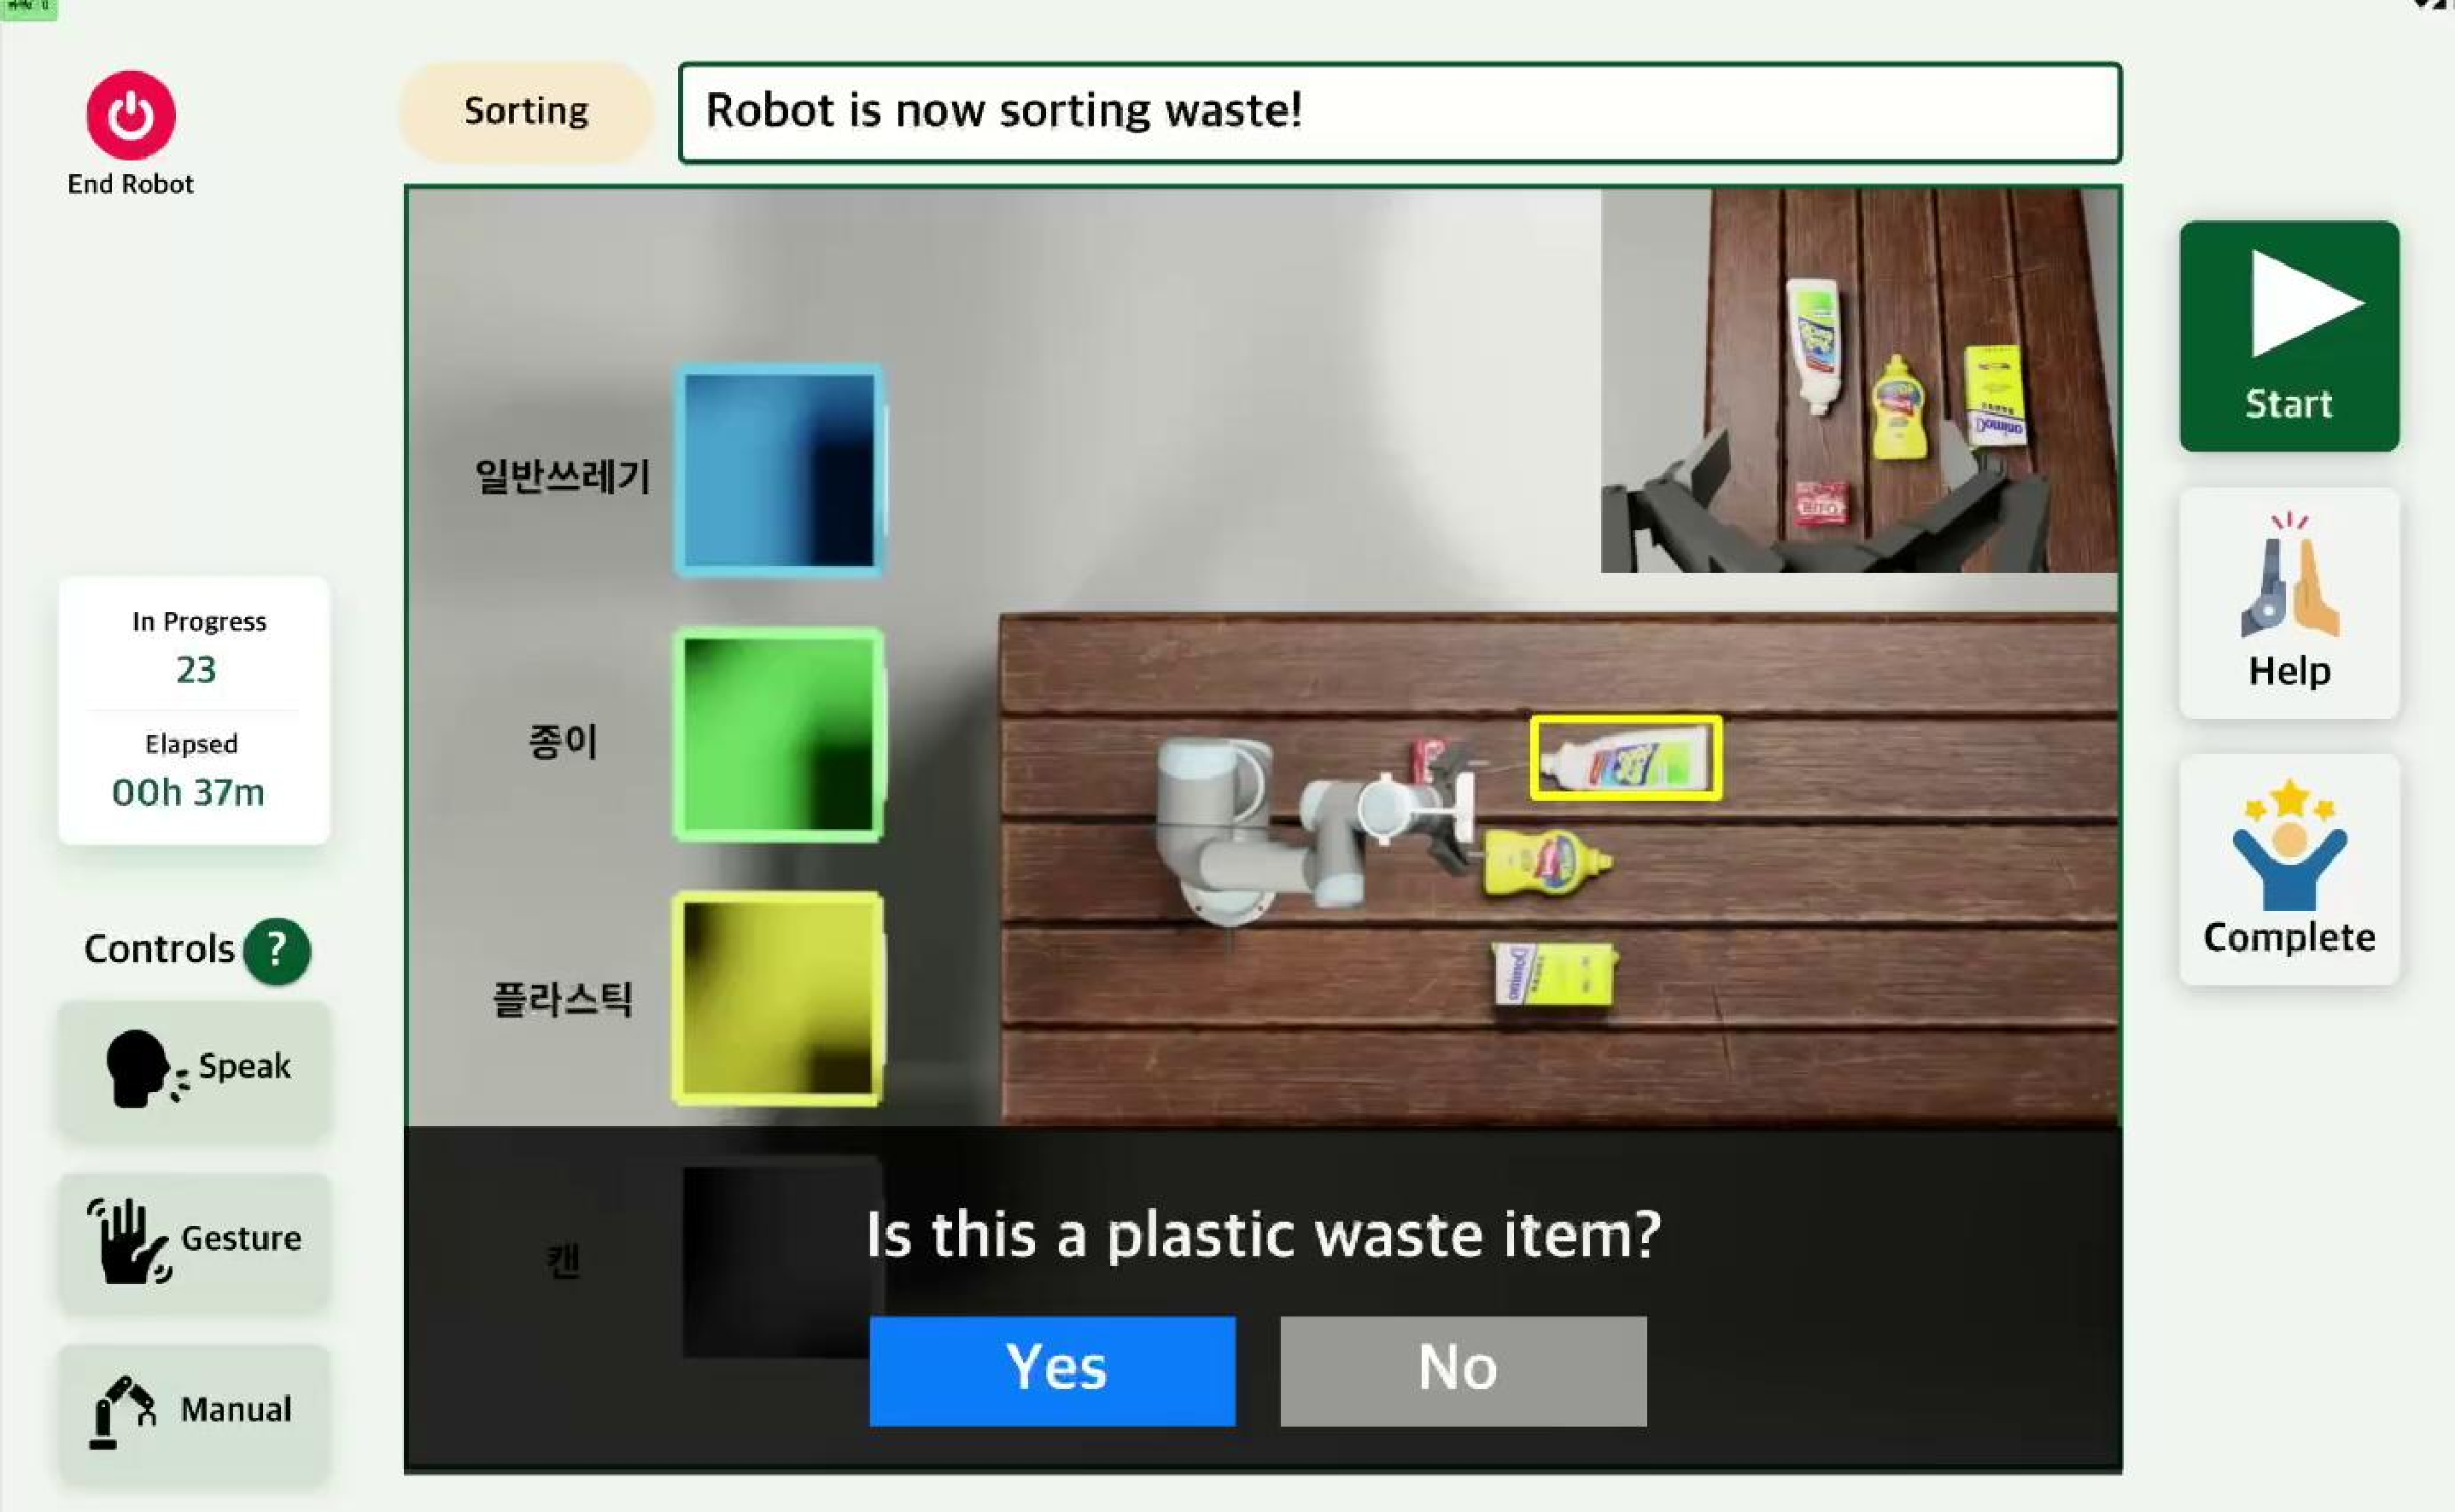
\includegraphics[width=\textwidth]{figures/intro_and_method/fig_interface_waste.pdf}
        \caption{Example of a waste sorting query}
        \label{fig:interface1}
    \end{subfigure}
    \quad
    \begin{subfigure}[b]{0.47\textwidth}
        \captionsetup{skip=0pt}
	    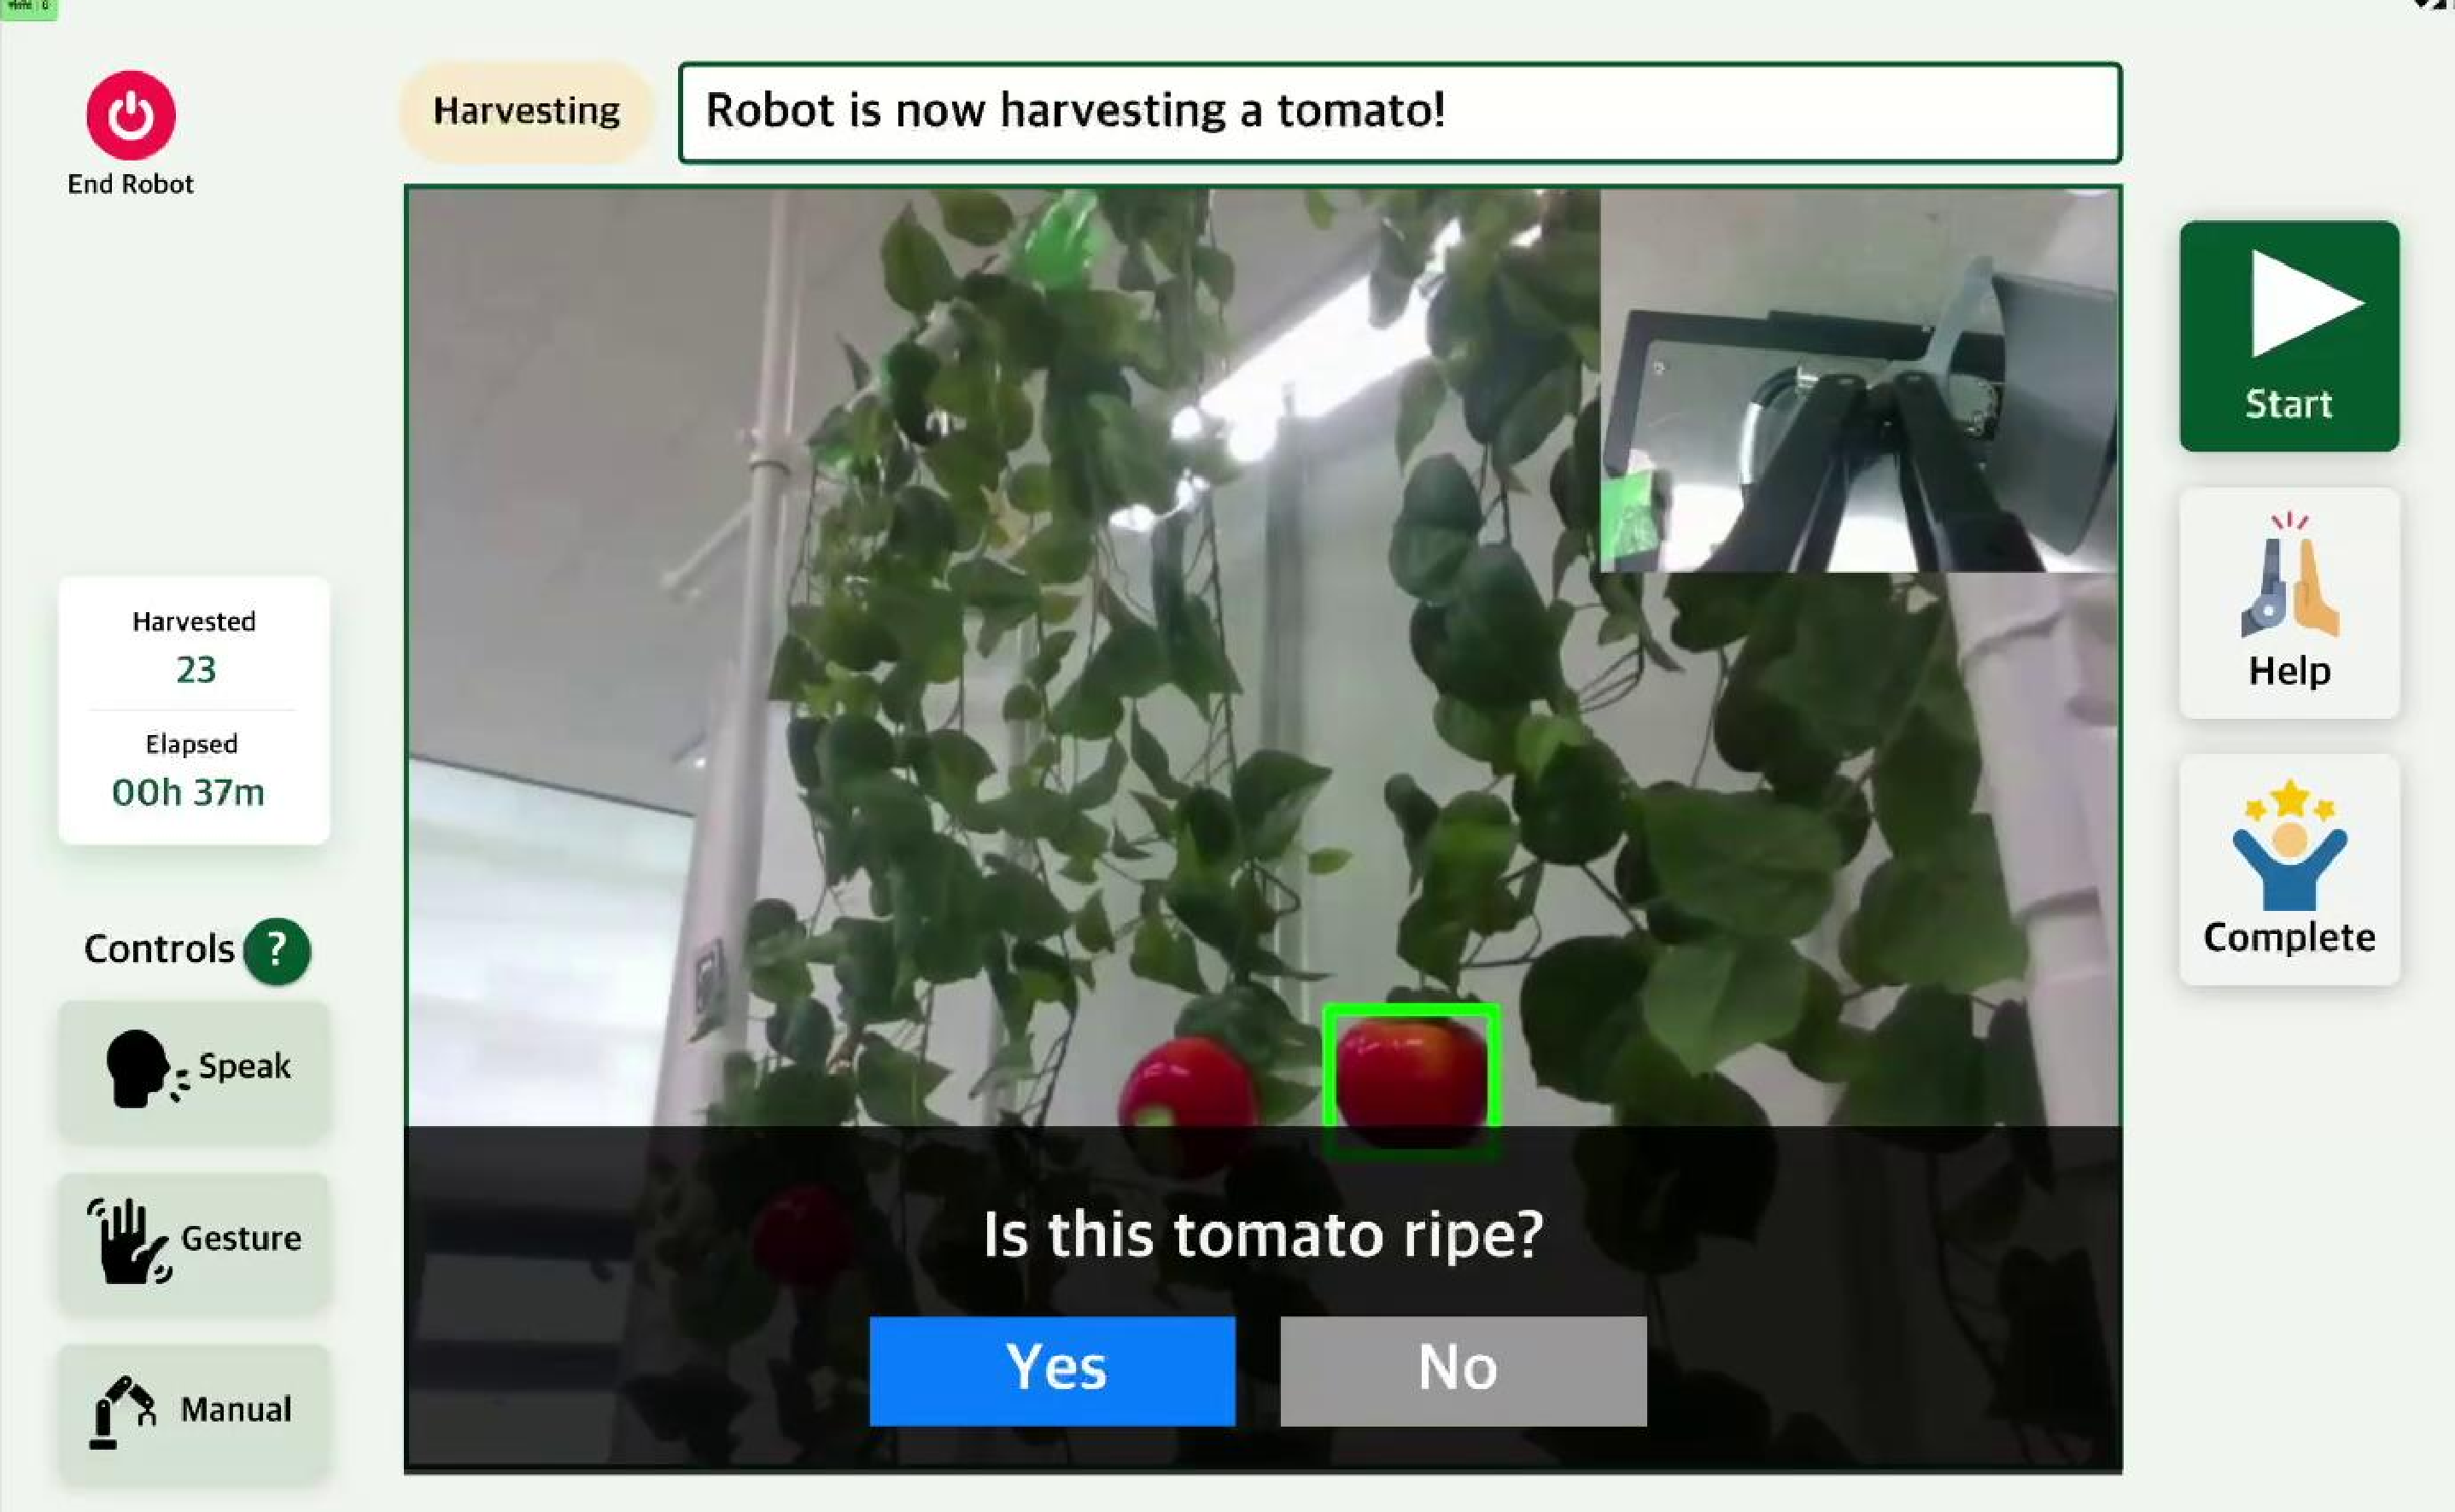
\includegraphics[width=\textwidth]{figures/intro_and_method/fig_interface_tomato.pdf}
        \caption{Example of a tomato harvesting query}
        \label{fig:interface2}
    \end{subfigure}
    \caption{Examples of the query interface used for human feedback. The interface visualizes the current observations of robot and highlights objects relevant to the queried state. Users provide binary feedback through the touchscreen interface to clarify task-relevant uncertainty. (a) The user identifies the category of a detected waste item in the waste sorting domain. (b) The user confirms the ripeness of a detected tomato in the tomato harvesting domain.}
  \label{fig:FM_UI}
  
  \end{center}
\end{figure*}
